\chapter{Постановка задачи декодирования сигналов}
\label{ch:intro}

В данной главе ставится общая задача декодирования временных рядов.
Приводится обзор стандартных методов анализа временных рядов.
Ставится задача построения оптимальной линейной авторегрессионной модели декодирования.
Приведен обзор широко используемых методов снижения размерности пространства, их обобщений и модификаций.

\section{Регрессионная модель в пространстве высокой размерности}

Задача декодирования формулируется следующим образом. 
Требуется построить регрессионную модель между объектами из двух пространств: $\bbX$ и $\bbY$.
Пространства обладают высокой, избыточной размерностью. 
Регрессионная модель оказывается неустойчивой.
Для построения простой, точной и устойчивой модели предлагается учесть наличие внутренней структуры обоих пространств. 
Применяются методы снижения размерности пространств для независимой и целевой переменной. 
Итоговая регрессионная модель строится путём согласования образов исходных объектов в низкоразмерном пространстве. 

Формализуем описанную задачу. 
Пусть $\bx \in \bbX \subset \bbR^n$~-- независимая переменная, $\by \in \bbY \subset \bbR^r$~-- целевая переменная.

\begin{definition}
	Назовём \textit{примером} пару $(\bx, \by)$, состоящую из реализации независимой переменной $\bx \in \bbX$ и целевой переменной $\by \in \bbY$. 
\end{definition}

\begin{definition}
	\textit{Выборкой} $\cD=(\bX, \bY)$ будем называть заданное множество примеров $\{(\bx_i, \by_i)\}_{i=1}^m$. Здесь $\bX \in \bbR^{m \times n}$~-- матрица независимой переменной, $\bY \in \bbR^{n \times k}$~-- матрица целевой переменной:
	\begin{equation*}
	\bX = [\bx_1, \dots, \bx_m]^{\T} =  [\bchi_1, \dots, \bchi_n]; \quad \bY = [\by_1, \dots, \by_m]^{\T} =  [\bnu_1, \dots, \bnu_r].
	\end{equation*}
	
	Столбцы~$\bchi_j, j=1, \dots, n$ матрицы~$\bX$ являются признаками объекта, столбцы~$\bnu_j, j=1, \dots, r$ матрицы ~$\bY$ являются целевыми столбцами.
	
\end{definition}

\begin{definition}
Назовём \textit{моделью} отображение $f: \bbX \rightarrow \bbY$ из пространства независимой переменной в пространство целевой переменной.
\end{definition}

Задача восстановления регрессии состоит в нахождении оптимальной модели $f^*$ по известной выборке $\cD$. Под оптимальностью понимается нахождение такой модели, которая бы доставляла минимум некоторой функции ошибки
\begin{equation}
	f^* = \argmin_f \cL(f, \bX, \bY).
	\label{ch1:eq:loss_min}
\end{equation}

Задача поиска оптимальной модели является задачей функциональной оптимизации. 
Для сужения пространства поиска моделей будем рассматривать параметрические модели $f(\bx, \bTheta)$, где $\bTheta$ являются \textit{параметрами модели}. 
Тогда задача~\eqref{ch1:eq:loss_min} сводится к задаче поиска набора оптимальных параметров
\begin{equation}
\bTheta^* = \argmin_{\bTheta} \cL(\bTheta, \bX, \bY).
\label{ch1:eq:loss_min_param}
\end{equation}

В данной диссертации рассматривается случай, когда размерность пространств~$\bbX$, $\bbY$ является избыточной. 
В таком случае решение задачи~\eqref{ch1:eq:loss_min_param} оказывается неустойчивым. 
Рассмотрим в качестве примера задачу восстановления линейной регрессии.

%%%%%%%%%%%%%%%%%%%%%%%%%%%%%%%%%%%%%%%%%%%%%%%%
\section{Задача декодирования временных рядов}
\label{ch1:time_series}
%%%%%%%%%%%%%%%%%%%%%%%%%%%%%%%%%%%%%%%%%%%%%%%%

Рассмотрим задачу декодирования временных рядов. 

\begin{definition}
Пусть $\bS = [\bs_1, \dots \bs_T]$~-- \textit{сегмент многомерного временного ряда}.
Вектор $\bs_t$ содержит значения временного ряда в момент времени $t$. 
В случае одномерного временного ряда $\bs_t$ является скаляром.
\end{definition}

\begin{definition}
	Назовём \textit{задачей декодирования временных рядов} задачу восстановления значений сегментов целевых временных рядов $\bS_y$ по сегментам наблюдаемых независимых временных рядов $\bS_x$.
\end{definition}

Если сегмент целевого временного ряда $\bS_y$ является продолжением наблюдаемого сегмента $\bS_x$ задача декодирования сводится к построению прогностическом модели временного ряда.
Для построения модели прогнозирования временных рядов широко используются два класса линейных методов: авторегрессионные модели~\cite{box2011time,hipel1994time} и модели скользящего среднего~\cite{box2011time,hipel1994time}. 
Авторегрессионные модели AR($p$) строят прогноз в виде линейной комбинации $p$ предыдущих значений временного ряда.
Модели скользящего среднего MA($q$) вместо предыдущих значений временного ряда используют комбинацию ошибок.
Модель ARMA($p$, $q$)~\cite{cochrane2005time} является комбинацией двух описанных подходов. 
ARMA($p$, $q$) задает модель как линейную комбинацию $p$ предыдущих значений временного ряда и $q$ предыдущих значений ошибок. 
Для нахождения оптимальных параметров $p$ и $q$ модели ARMA используются автокорреляционная и частная автокорреляционная функции. 

Модель ARMA используется для стационарных временных рядов, отвечающим строгим статистическим предположениям. 
На практике встречается огромное количество нестационарных временных рядов подверженных тренду, сезонности или цикличности.
Модель ARIMA($p$, $d$, $q$)~\cite{cochrane2005time} обобщает модель ARMA для случая нестационарных временных рядов.
ARIMA берёт разности порядка $d$ от исходного временного ряда для достижения стационарности данных. 
При этом на практике оказывается достаточным положить $d = 1$.
Заметим, что при $d = 0$ модель ARIMA эквивалентна модели ARMA. 
Полезным обобщение модели ARIMA явялется модель AFRIMA~\cite{galbraith2001autoregression}. 
Модель позволяет задать параметр $d$ в виде вещественного числа.

Модель ARIMA плохо справляется с сезонными временными рядами.
В работе~\cite{box2011time} была предложена модель SARIMA, которая вводит в модель учет сезонной компоненты.

Задача декодирования временных рядов декомпозируется на следующие подзадачи.
\begin{itemize}
	\item Порождение признакового пространства. 
	Данный этап включает в себя процедуру извлечения признаков из исходных значений сигналов. 
	Процедура порождения признакового пространства может быть основана на экспертных знания или же являться моделью машинного обучения. 
	Данная подзадача подробно рассмотрена в~\autoref{ch:metamodels}.
	
	\item Снижение размерности пространства или выбор признаков. 
	Исходные временные ряды, а также порожденное признаковое пространство оказывается избыточным, что приводит к избыточности и неустойчивости модели. 
	Алгоритмы снижения размерности и выбора признаков подробно изложены в~\autoref{ch:pls} и~\autoref{ch:qpfs}.
	
	\item Построение модели.
	После нахождения оптимального низкоразмерного представления исходных данных ставится задача выбора оптимальной модели декодирования.
\end{itemize}

%%%%%%%%%%%%%%%%%%%%%%%%%%%%%%%%%%%%%%%%%%%%%%%%
\section{Линейная регрессия для многомерных сигналов}
\label{ch1:sec_lin_reg}
%%%%%%%%%%%%%%%%%%%%%%%%%%%%%%%%%%%%%%%%%%%%%%%%

Предполагается, что между объектами $\bx$ и ответами $\by$ существует зависимость вида
\begin{equation}
	\by = f(\bx, \bTheta) + \boldsymbol{\varepsilon},
	\label{ch1:eq:reg_model}
\end{equation}
где $f$~-- параметрическая модель регрессионной зависимости, $\bTheta$~-- пространство параметров модели, $\bepsilon \in \bbR^{m}$~-- вектор регрессивных остатков. 
Необходимо восстановить зависимость $f$ по заданной наблюдаемой выборке~$\mathcal{D}$.

Предположим, что зависимость $f(\bx, \bTheta)$ линейная:
\begin{equation}
	\by = f(\bx, \bTheta) + \bepsilon = \bTheta \bx+ \bepsilon,
	\label{ch1:eq:lin_reg_model}
\end{equation}
\noindent где $\bTheta \in \bbR^{r \times n}$~-- матрица параметров модели.

Необходимо найти матрицу параметров модели~$\bTheta$ при известной выборке~$\mathcal{D} = \left( \bX, \bY \right)$.
Оптимальные параметры~$\bTheta$ определяются минимизацией функции ошибки $\cL(\bTheta, \bX, \bY)$.
При решении задачи линейной регрессии в качестве такой функции ошибки рассматривается квадратичная функция потерь:
\begin{equation}
	\cL(\bTheta, \bX, \bY) = {\left\| \underset{m \times r}{\mathbf{Y}}  - \underset{m \times n}{\bX} \cdot \underset{r \times n}{\bTheta}^{\T} \right\| }_2^2 \rightarrow\min_{\bTheta}.
	\label{ch1:eq:l2_loss_function}
\end{equation}
Решением~\eqref{ch1:eq:l2_loss_function} является следующая матрица:
\begin{equation*}
	\bTheta = \bY^{\T} \bX (\bX^{\T} \bX)^{-1}.
\end{equation*}

Наличие линейной зависимости между столбцами матрицы~$\bX$ приводит к неустойчивому решению задачи оптимизации~\eqref{ch1:eq:l2_loss_function}.
Если существует вектор~$\boldsymbol{\alpha} \neq \bZero_n$ такой, что $\bX \boldsymbol{\alpha}= \bZero_m$, то добавление~$\boldsymbol{\alpha}$ к любому столбцу матрицы~$\bTheta$ не меняет значение функции потерь~$\cL(\bTheta, \bX, \bY)$.
В этом случае матрица~$\bX^{\T} \bX$ близка к сингулярной и не обратима.
Чтобы избежать сильной линейной зависимости между признаками, в данной работе исследуются методы снижения размерности и выбора признаков.


%%%%%%%%%%%%%%%%%%%%%%%%%%%%%%%%%%%%%%%%%%%%%%%%
\section{Обзор методов снижения размерности для задачи декодирования}
\label{ch1:sec_lin_reg}
%%%%%%%%%%%%%%%%%%%%%%%%%%%%%%%%%%%%%%%%%%%%%%%%
Методы снижения размерности позволяют найти низкоразмерное представление исходных данных. 
Найденное представление используется для построения предсказательной модели.
При этом метод снижения размерности может учитывать как зависимости в исходном объекте~$\bx$, так и в целевой переменной~$\by$.

\vspace{0.5cm}
\textbf{Метод главных компонент для задачи декодирования.}
Для устранения линейной зависимости и снижения размерности входного пространства объектов широко используется метод главных компонент~(principal component analysis, PCA). 
Метод PCA находит низкоразмерное представление матрицы~$\bX = \bT \bP^{\T}$, такое что новое представление~$\bT \in \bbR^{m \times l}$ содержит максимальную долю дисперсии исходной матрицы.
При этом матрица отображения $\bP \in \bbR^{n \times l}$ является ортогональной ($\bP^{\T} \bP = \bI$) и содержит правые собственные вектора матрицы ковариаций $\bX^{\T} \bX$.

Метод PCA является базовым методом снижения размерности пространства. 
Существует множество модификаций базового метода.
Bероятностный PCA~\cite{tipping1999probabilisticpca} рассматривает задачу снижения размерности в терминах вероятностной модели, решая задачу с помощью вариационного EM алгоритма. 
Разреженный PCA~\cite{zou2006sparsepca} вводит в постановку задачи lasso регуляризацию для того, чтобы сделать матрицу отображения~$\bP$ разреженной и более интерпретируемой.
Нелинейный ядерный PCA~\cite{scholkopf1997kernelpca} отображает исходные данные с помощью нелинейного отображения и использует RKHS для решения исходной задачи.

После нахождения матрицы отображения $\bP$ задача~\eqref{ch1:eq:l2_loss_function} принимает вид

\begin{equation}
	\cL(\bB, \bT, \bY) = {\left\| \underset{m \times r}{\mathbf{Y}}  - \underset{m \times l}{\bT} \cdot \underset{r \times l}{\bB}^{\T} \right\| }_2^2 \rightarrow\min_{\bB}.
	\label{ch1:eq:l2_loss_function_pca}
\end{equation}

Модель прогнозирования~\eqref{ch1:eq:lin_reg_model} в случае снижения размерности с помощью PCA принимает вид:
\begin{equation}
	\by = \bB \bt + \bepsilon = \bB \bP \bx + \bepsilon = \bTheta \bx + \bepsilon, \, \text{ где } \bTheta = \bB \bP.
	\label{ch1:eq:lin_reg_model_pca}
\end{equation}

\vspace{0.5cm}
\textbf{Метод частичных наименьших квадратов для задачи декодирования.}
Основным недостатком метода PCA является отсутствие учёта взаимосвязи между признаками~$\bchi_j$ и целевыми векторами~$\bnu_j$.
Алгоритм частичных наименьших квадратов проецирует матрицу объектов~$\bX$ и матрицу ответов~$\bY$ в скрытое пространство малой размерностью~$l$ ($l < n$).
Алгоритм PLS находит в скрытом пространстве матрицы~$\bT, \bU \in \bbR^{m \times l}$, которые лучше всего описывают оригинальные матрицы~$\bX$ и~$\bY$. 
При этом PLS максимизирует ковариацию между столбцами $\bt$ и $\bu$ матриц $\bT$ и $\bU$ соответственно.

Алгоритм PLS был впервые предложен в работах~\cite{wold1975path,wold1984collinearity,wold1982pls}. Подробное описание алгоритма приведено в работах~\cite{geladi1986partial,geladi1988notes,de1993simpls,vinzi2010handbook,brereton2014partial}.
В работах~\cite{rosipal2005overview,rosipal2011nonlinear} приведен обзор обобщений базовой модели PLS.
В работе~\cite{chun2010sparse} приведена модификация алгоритма PLS для получения разреженного набора признаков. 
 

Матрица объектов $\bX$ и целевая матрица $\bY$ проецируются на латентное пространство следующим образом:

\begin{align}
	\label{ch1:eq:PLS_X}
	\underset{m \times n}{\bX} 
	&= \underset{m \times l}{\bT} \cdot \underset{l \times n}{\bP^{\T}} + \underset{m \times n}{\bF} 
	= \sum_{k=1}^l \underset{m \times 1}{\bt_k} \cdot \underset{1 \times n}{\bp_k^{\T}} + \underset{m \times n}{\bF},\\
	\label{ch1:eq:PLS_Y}
	\underset{m \times r}{\bY} 
	&= \underset{m \times l}{\bU} \cdot \underset{l \times r}{\bQ^{\T}} + \underset{m \times r}{\bE}
	=  \sum_{k=1}^l  \underset{m \times 1}{\bu_k} \cdot \underset{1 \times r}{\bq_k^{\T}} +  \underset{m \times r}{\bE}.
\end{align}

Здесь $\bT$ и $\bU$~-- образы исходных матриц в скрытом пространстве, причём столбцы матрицы $\bT$ ортогональны; $\bP$ и $\bQ$~-- матрицы перехода; $\bE$ и $\bF$~-- матрицы остатков. 
Алгоритм PLS максимизирует линейную зависимость между столбцами матриц~$\bT$ и~$\bU$
\begin{equation*}
	\bU \approx \bT \bB, \quad \bB = \text{diag}(\beta_k), \quad \beta_k = \bu_k^{\T}\bt_k / (\bt_k^{\T}\bt_k)
\end{equation*}

Алгоритм решает следующую оптимизационную задачу:
\begin{equation}
	\max_{\|\bp\|_{2}=\|\bq\|_{2}=1}[ \text{cov}(\bX \bp, \bY \bq)^{2}] = \max_{\bp, \bq} \frac{\bp^{\T} \bX^{\T} \bY \bq}{\sqrt{\bp^{\T} \bp} \sqrt{\bq^{\T} \bq}}.
	\label{ch1:eq:pls_max_cov}
\end{equation}

Детальное описание алгоритма PLS с доказательством его корректности приведено в~\autoref{ch:pls}.

Для демонстрации разницы между алгоритмами PCA, PLS был проведен модельный эксперимент для случая, когда размерности пространств объектов, ответов и латентного пространства равны 2 ($n = r = l = 2$).
На Рис.~\ref{ch1:fig:pls_toy_example} показаны результаты работы методов. 
Синими и зелёными точками изображены объекты~$\bx_i$ и целевые переменные~$\by_i$. 
Точки $\bX$ сгенерированы из нормального распределения с нулевым матожиданием. 
Точки $\bY$ линейным образом зависят от второй  главной компоненты $pc_2$ матрицы $\bX$ и не зависят от первой главной компоненты $pc_1$.
Красным контуром показаны линии уровня матриц ковариаций распределений. 
Черным изображены единичные окружности. 
Красные стрелки соответствуют главным компонентам матриц~$\bX$ и~$\bY$. 
Черные стрелки соответствуют векторам матриц~$\bW$ и~$\bC$ алгоритма PLS. 
Данные матрицы содержат вектора, являющиеся аналогами главных компонент алгоритма PCA.
Учёт взаимной связи между матрицами~$\bX$ и~$\bY$ отклоняет вектора~$\bw_k$ и~$\bc_k$ от направления главных компонент. 
\begin{figure}[h]
	\centering
	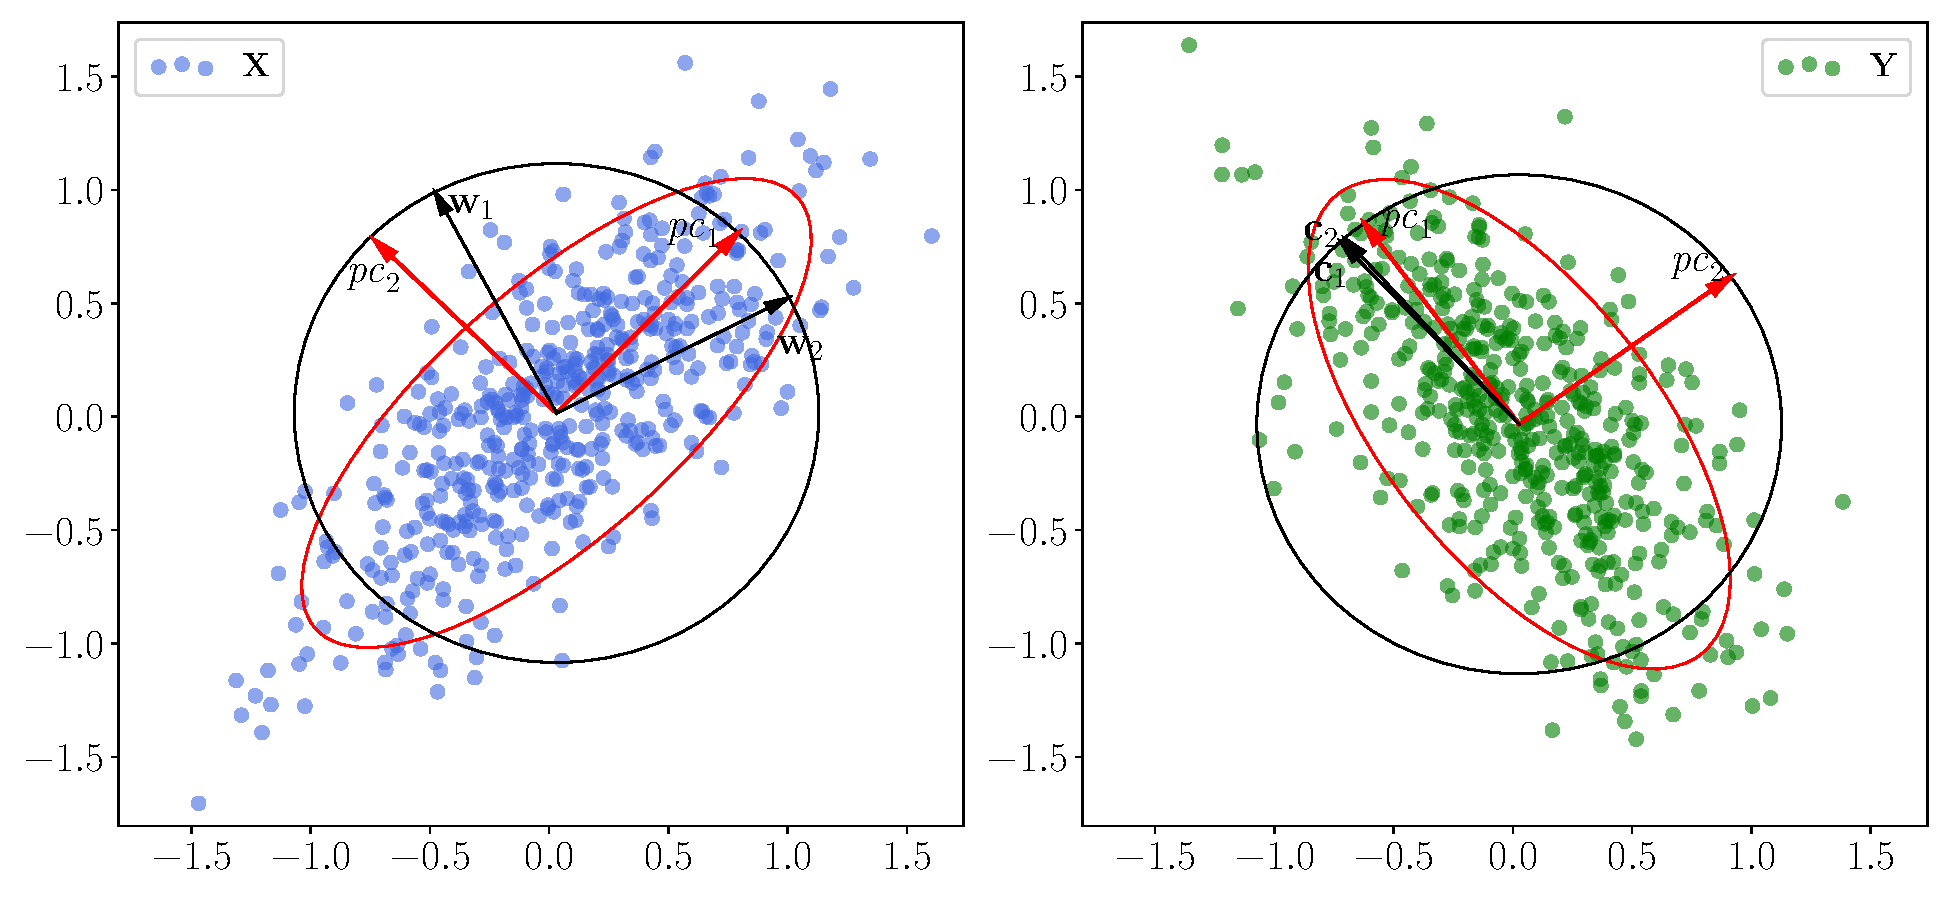
\includegraphics[width=\linewidth]{figs/ch1/pls_toy_example}
	\caption{Модельный пример работы алгоритмов PCA и PLS}
	\label{ch1:fig:pls_toy_example}
\end{figure}

При снижении размерности пространств до одного признака алгоритм PCA выберет первую главную компоненту $pc_1$, отбросив компоненту $pc_2$, так как первая компонента объясняет большую части дисперсии исходной матрицы $\bX$. 
При этом матрица $\bY$ не зависит от $pc_1$. 
Тем самым финальная модель окажется не оптимальной.
Алгоритм PLS позволяет побороться с данной проблемой.

\vspace{0.5cm}
\textbf{Канонический анализ корреляций для задачи декодирования.}
Канонический корреляционный анализ (canonical correlation analysis, CCA) широко применяется для поиска взаимосвязи между двумя наборами переменных~\cite{hotelling1992relations,anderson1962introduction}. 
Оптимизационная задача CCA похожа на оптимизационную задачу PLS~\eqref{ch1:eq:pls_max_cov} с той лишь разницей, что вместо максимизации ковариации CCA максимизирует корреляцию:
\begin{equation}
	\max_{\|\bp\|_{2}=\|\bq\|_{2}=1}[ \text{corr}(\bX \bp, \bY \bq)^{2}] = \max_{\bp, \bq} \frac{\bp^{\T} \bX^{\T} \bY \bq}{\sqrt{\bp^{\T} \bX^{\T}  \bX \bp} \sqrt{\bq^{\T} \bY^{\T}  \bY\bq}}.
	\label{ch1:eq:cca_max_corr}
\end{equation}

На Рис.~\ref{ch1:fig:cca_toy_example} показан результат работы алгоритма. 
Основное различие состоит в том, что вектора $\bc_1$ и $\bc_2$ в данном случае становятся ортогональными.

\begin{figure}[h]
	\centering
	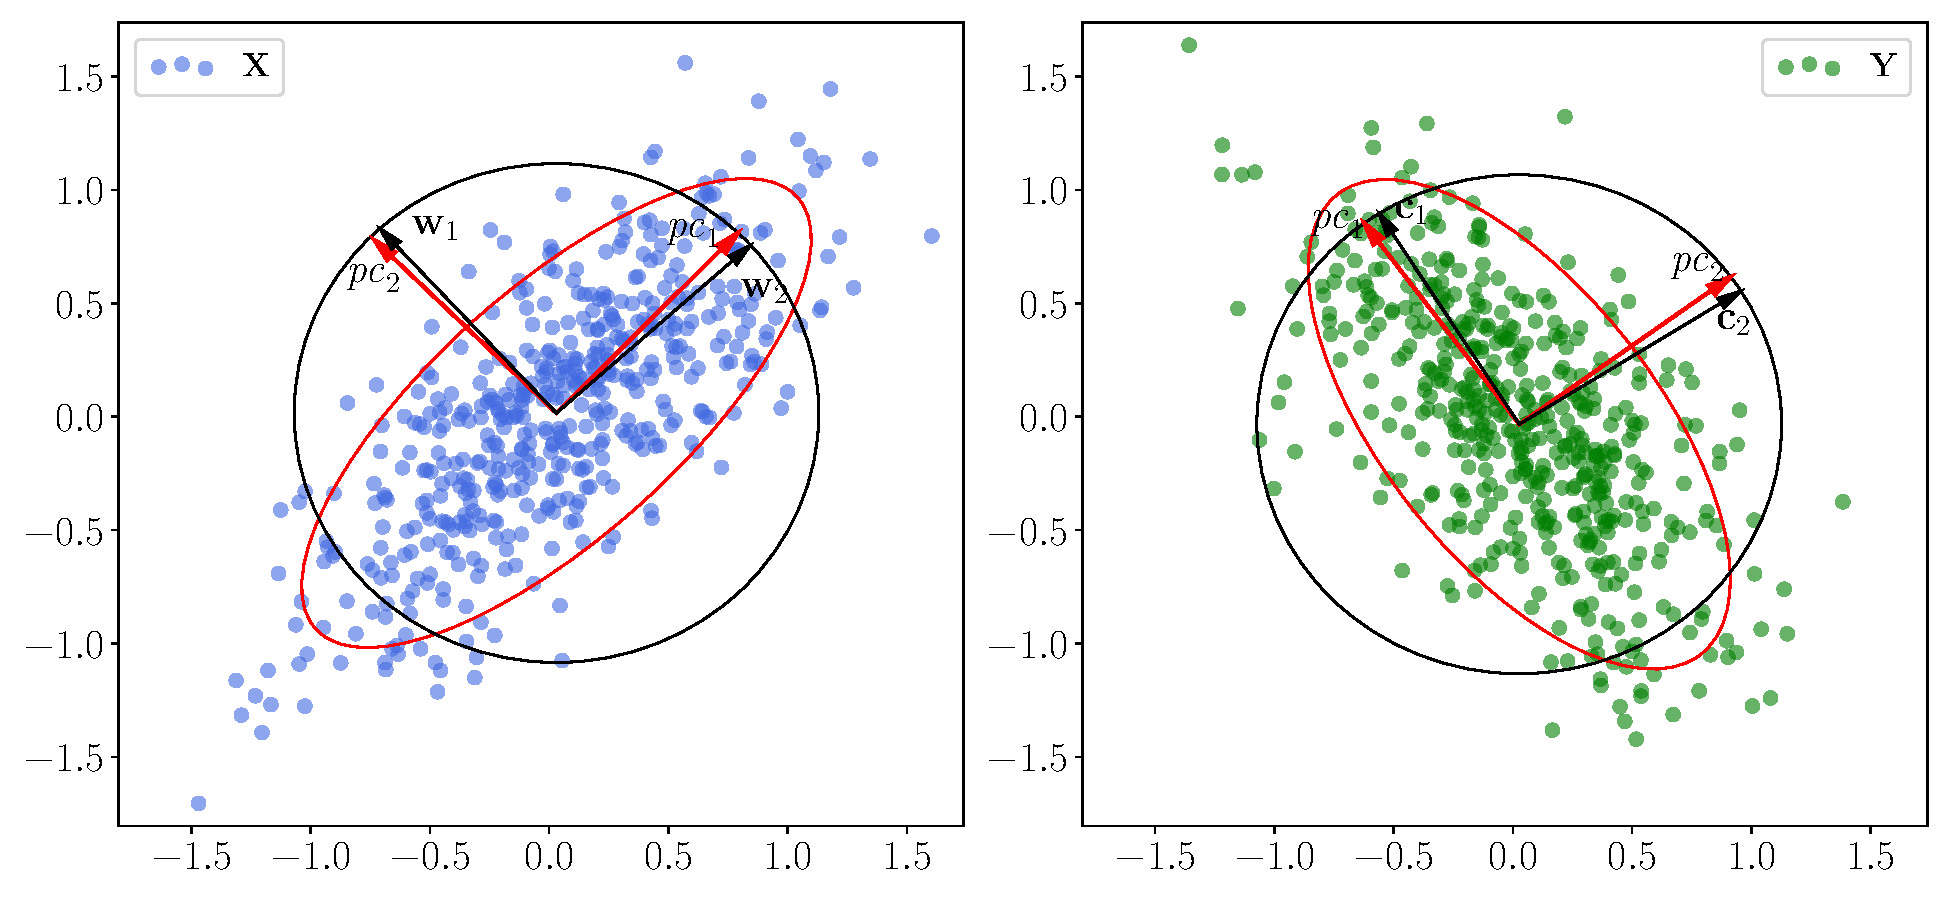
\includegraphics[width=\linewidth]{figs/ch1/cca_toy_example}
	\caption{Модельный пример работы алгоритмов PCA и CCA}
	\label{ch1:fig:cca_toy_example}
\end{figure}

В Таблице~\ref{ch1:tbl:toy_example_results} приведены значения квадратичной ошибки $\mathcal{L}(\bTheta, \bX, \bY)$ для алгоритмов линейной регрессии, PCA и PLS.
Линейная регрессия отлично справляется с данной задачей.
Ошибка алгоритма PCA наибольшая, что подтверждает факт, что для данной ситуации алгоритм не находит нужных зависимостей в пространстве целевой переменной. 
Алгоритмы PLS и CCA показывают схожие результаты.

\begin{table}[]
	\centering
	\begin{tabular}{|c|c|c|c|}
		\hline
		\textbf{Линейная регрессия} & \textbf{PCA}   & \textbf{PLS}  &  \textbf{CCA}  \\ \hline
		0.01 &  0.24   &  0.13 &  0.13 \\ \hline
	\end{tabular}
	\caption{Средняя квадратичная ошибка на модельном примере для алгоритмов линейной регрессии, PCA, PLS, CCA}
	\label{ch1:tbl:toy_example_results}
\end{table} 


Нелинейный ядерный CCA~\cite{akaho2006kernel,melzer2001nonlinear,bach2002kernel,hardoon2004canonical} является обобщением базового метода. 
CCA и ядерный CCA широко используются для задач обучения без учителя~\cite{hardoon2007unsupervised,vinokourov2003inferring}. 
Метод имеет область применения от анализа хемометрических~\cite{montanarella1995chemometric} и биологических~\cite{vert2003graph} данных до обработки естественного языка~\cite{haghighi2008learning,dhillon2011multi}, аудиосигналов~\cite{choukri1986adaptation,rudzicz2010adaptive} и компьютерного зрения~\cite{kim2007tensor}.

В работе~\cite{andrew2013deep} был впервые предложено обобщение алгоритма CCA, работающего с нейросетями. 
Предложенный алгоритм DeepCCA максимизирует корреляцию между представлениями, полученными на выходе нейросети:
\begin{multline}
	\max_{\|\bp\|_{2}=\|\bq\|_{2}=1}\left[ \text{corr}(\mathbf{f}(\bX, \bW_{\bx}) \cdot \bp, \mathbf{g}(\bY, \bW_{\by}) \cdot \bq)^{2}\right] = \\ = \max_{\bp, \bq} \frac{\bp^{\T} \mathbf{f}(\bX, \bW_{\bx})^{\T} \mathbf{g}(\bY, \bW_{\by}) \bq}{\sqrt{\bp^{\T} \mathbf{f}(\bX, \bW_{\bx})^{\T}  \mathbf{f}(\bX, \bW_{\bx}) \bp} \sqrt{\bq^{\T} \mathbf{g}(\bY, \bW_{\by})^{\T}  \mathbf{g}(\bY, \bW_{\by}) \bq}}.
	\label{ch1:eq:depp_cca_max_corr}
\end{multline}
Здесь $\mathbf{f}(\bX, \bW_{\bx})$ и $\mathbf{g}(\bY, \bW_{\by})$~-- нелинейные проекции исходных и целевых объектов.
В статье~\cite{wang2015deep} приведен обширный обзор модификаций нейросетевого CCA для работы с многовидовыми данными.
Главным недостатком нейросетевого CCA является вычислительная сложность. 
В работе~\cite{chang2018scalable} предложена релаксация исходного лосса, которая способна масштабироваться под работу с большими глубокими моделями.

\vspace{0.5cm}
\textbf{Тензорные линейные методы для задачи декодирования.}
Если исходный объект $\bx$ являеттся вектором, а тензором более высокого порядка, то для построения модели тензор может быть вытянут в вектор~\cite{cichocki2009nonnegative}. 
В таком случае модель не учитывает имеющиеся зависимости между различными направлениями исходного тензора.
Для учета таких зависимостей используются тензорные версии алгоритма PLS~\cite{zhao2012higher,eliseyev2013recursive,eliseyev2016penalized}.


\vspace{0.5cm}
\textbf{Многомодальные данные в задаче декодирования.}
Исходный объект может иметь несколько модальностей. 
Примерами таких модальностей могут быть выровненные аудио и видео~\cite{kidron2005pixels,chaudhuri2009multi}, аудио и артикуляция~\cite{arora2012kernel}, изображение и текстовая аннотация~\cite{hardoon2004canonical,socher2010connecting,hodosh2013framing}, параллельный корпус текстов~\cite{vinokourov2003inferring,haghighi2008learning,ap2014autoencoder,faruqui2014improving}.

В случае если для каждого объекта имеется более двух модальностей, то для построения скрытого пространства для каждого из них применяются два класса подходов. 
Первый подход состоит в построении скрытого пространства для каждой пары модальностей объекта~\cite{masci2013multimodal,rajendran2015bridge}. 
Второй же подход состоит в построении общего единого скрытого пространства для всех модальностей~\cite{kumar2011co,sharma2012generalized}.